\newpage
\section{Device Partitioning Example}

This example illustrates how the device will be partitioned accordingly to the parameters passed to the \textbf{clCreateSubDevices()} function. (See \textbf{OpenCL (\ref{Code:DevicePartitioning}}) on page \pageref{Code:DevicePartitioning})
The architecture used in the example is a 2 processor (4 cores each) with L3 chache shared among the cores. 

\begin{figurehere}
  {\centering
 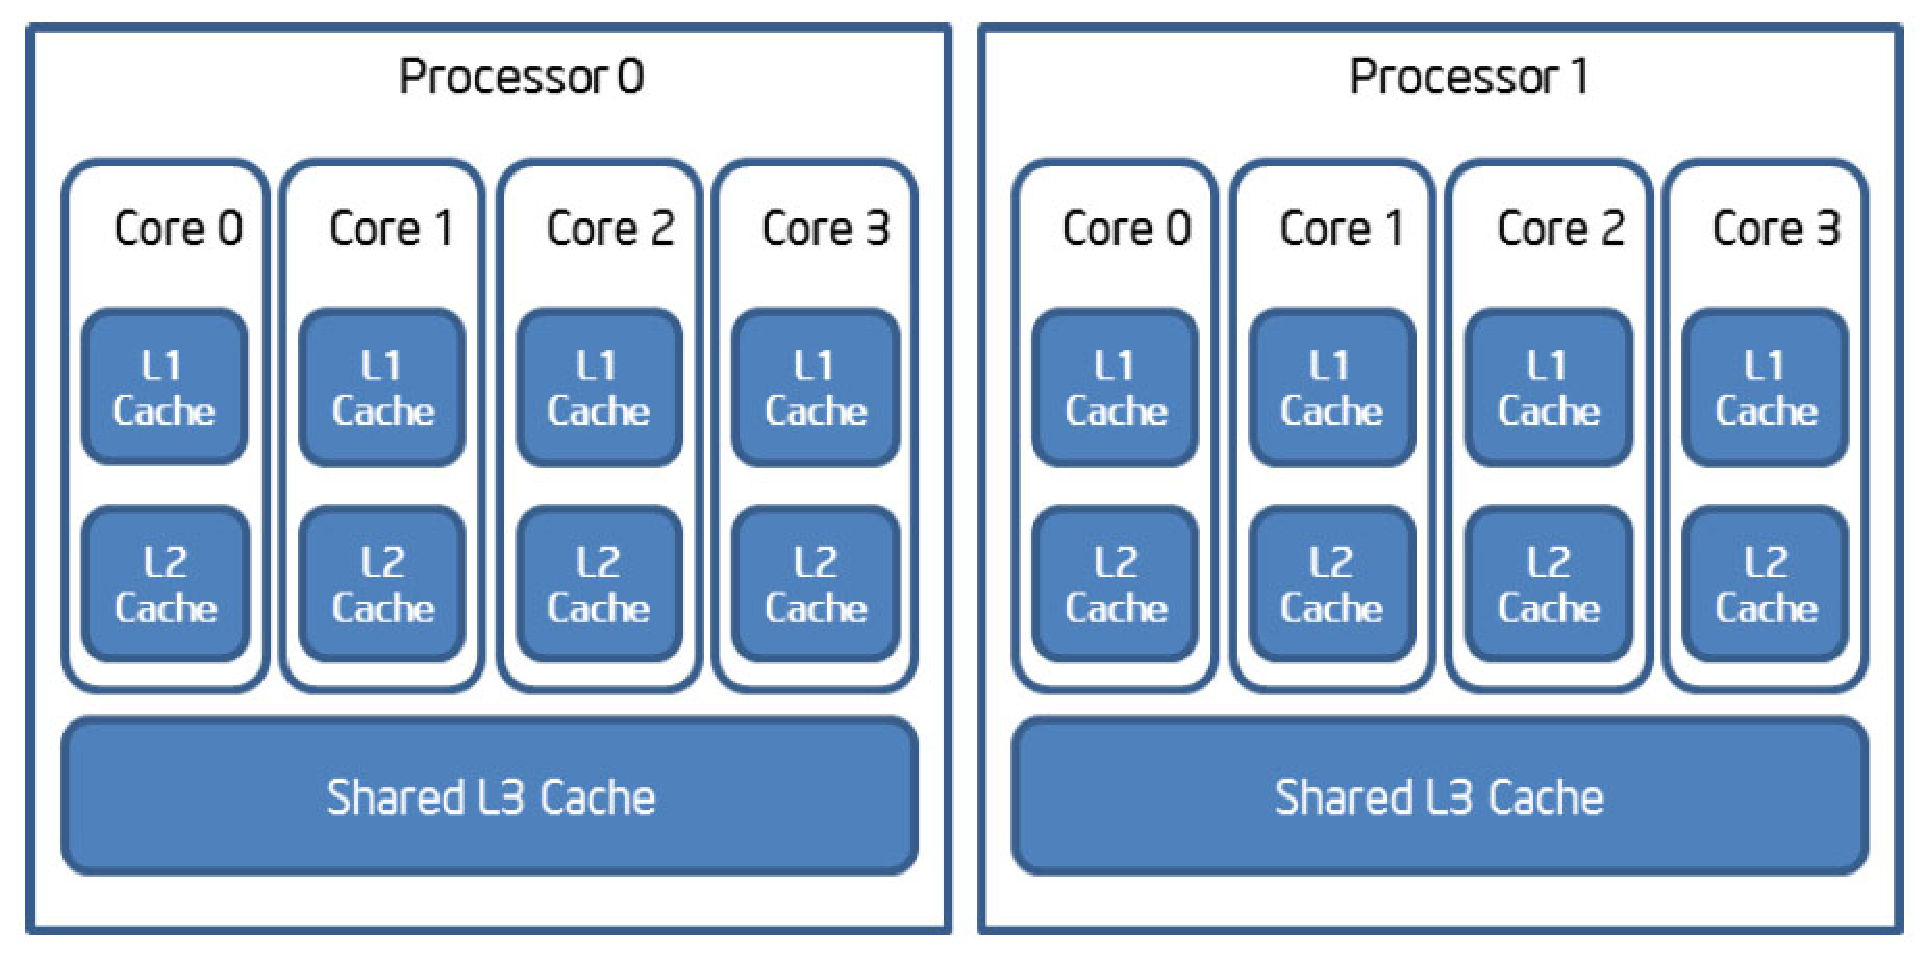
\includegraphics[height=4cm]{./eps/ExampleArchitecture_A.eps}
 \caption{Architecure used in the example}}
 \label{fig:AppAArch}
\end{figurehere}

\begin{tablehere}
{\footnotesize
����\begin{tabular}{|p{8cm}|p{3cm}|p{5cm}|}\hline
Property List&Description&Result on the Example Target Machine\\ \hline
{ CL\_DEVICE\_PARTITION\_EQUALLY, 8, 0 }&
Partition the device into as many sub-devices as possible, each with 8 compute units.&
2 sub-devices, each with 8 threads.\\ \hline
{ CL\_DEVICE\_PARTITION\_EQUALLY, 4, 0 }&
Partition the device into as many sub-devices as possible, each with 4 compute units.&
4 sub-devices, each with 4 threads.\\ \hline
{ CL\_DEVICE\_PARTITION\_EQUALLY, 32, 0 }&
Partition the device into as many sub-devices as possible, each with 32 compute units.&
Error! 32 exceeds the CL\_DEVICE\_PARTITION\_MAX\_ COMPUTE\_UNITS.\\ \hline
{ CL\_DEVICE\_PARTITION\_BY\_COUNTS, 3, 1, CL\_DEVICE\_PARTITION\_BY\_COUNTS\_LIST\_END, 0 }&
Partition the device into two sub-devices, one with 3 compute units and one with 1 compute unit.&
1 sub-device with 3 threads and 1 sub-device with 1 thread.\\ \hline
{ CL\_DEVICE\_PARTITION\_BY\_COUNTS, 2, 2, 2, 2 CL\_DEVICE\_PARTITION\_BY\_COUNTS\_LIST\_END, 0 }&
Partition the device into four sub-devices, each with 2 compute units.&
4 sub-devices, each with 2 threads.\\ \hline
{ CL\_DEVICE\_PARTITION\_BY\_COUNTS, 3, 1, CL\_DEVICE\_PARTITION\_BY\_COUNTS\_LIST\_END, 0 }&
Partition the device into two sub-devices, one with 3 compute units and one with 1 compute unit.&
1 sub-device with 3 threads and 1 sub-device with 1 threads.\\ \hline
{ CL\_DEVICE\_PARTITION\_BY\_AFFINITY\_DOMAIN,
CL\_DEVICE\_AFFINITY\_DOMAIN\_NUMA,
0 }&
Partition the device into sub-devices that share a NUMA node.&
2 sub-devices with 8 threads each. Each sub-device is located on its own NUMA node.\\ \hline
{ CL\_DEVICE\_PARTITION\_BY\_AFFINITY\_DOMAIN,
CL\_DEVICE\_AFFINITY\_DOMAIN\_L1\_CACHE,
0 }&
Partition the device into sub-devices that share an L1 cache.&
8 sub-devices with 2 threads each. The L1 cache is not shared in our example machine.\\ \hline
{ CL\_DEVICE\_PARTITION\_BY\_AFFINITY\_DOMAIN,
CL\_DEVICE\_AFFINITY\_DOMAIN\_L2\_CACHE,
0 }&
Partition the device into sub-devices that share an L2 cache.&
8 sub-devices with 2 thread each. The L2 cache is not shared in our example machine.\\ \hline
{ CL\_DEVICE\_PARTITION\_BY\_AFFINITY\_DOMAIN,
CL\_DEVICE\_AFFINITY\_DOMAIN\_L3\_CACHE,
0 }&
Partition the device into sub-devices that share an L3 cache.&
2 sub-devices with 8 threads each. The L3 cache is shared among all 8 threads within each processor.\\ \hline
{ CL\_DEVICE\_PARTITION\_BY\_AFFINITY\_DOMAIN,
CL\_DEVICE\_AFFINITY\_DOMAIN\_L4\_CACHE,
0 }&
Partition the device into sub-devices that share an L4 cache.&
Error! There is no L4 cache.\\ \hline
{ CL\_DEVICE\_PARTITION\_BY\_AFFINITY\_DOMAIN,
CL\_DEVICE\_AFFINITY\_DOMAIN\_NEXT\_PARTITIONABLE,
0 }&
Partition the device based on the next partitionable domain. In this case, it is NUMA.&
2 sub-devices with 8 threads each. Each sub-device is located on its own NUMA node.\\ \hline
����\end{tabular}}
\caption{Device Partitioning Examples (Source: \textit{OpenCL Device Fission for CPU Performance, Intel Corporation})}
	\label{tab:AppAExample}
\end{tablehere}
